% 
% Annual Cognitive Science Conference
% Sample LaTeX Paper -- Proceedings Format
% 

% Original : Ashwin Ram (ashwin@cc.gatech.edu)       04/01/1994
% Modified : Johanna Moore (jmoore@cs.pitt.edu)      03/17/1995
% Modified : David Noelle (noelle@ucsd.edu)          03/15/1996
% Modified : Pat Langley (langley@cs.stanford.edu)   01/26/1997
% Latex2e corrections by Ramin Charles Nakisa        01/28/1997 
% Modified : Tina Eliassi-Rad (eliassi@cs.wisc.edu)  01/31/1998
% Modified : Trisha Yannuzzi (trisha@ircs.upenn.edu) 12/28/1999 (in process)
% Modified : Mary Ellen Foster (M.E.Foster@ed.ac.uk) 12/11/2000
% Modified : Ken Forbus                              01/23/2004
% Modified : Eli M. Silk (esilk@pitt.edu)            05/24/2005
% Modified : Niels Taatgen (taatgen@cmu.edu)         10/24/2006
% Modified : David Noelle (dnoelle@ucmerced.edu)     11/19/2014
% Modified : Roger Levy (rplevy@mit.edu)     12/31/2018



%% Change "letterpaper" in the following line to "a4paper" if you must.

\documentclass[10pt,letterpaper]{article}

\usepackage{cogsci}

% \cogscifinalcopy % Uncomment this line for the final submission 

% \usepackage{times}
% \cogscifinalcopy % Uncomment this line for the final submission 


% \usepackage{pslatex}
\usepackage{times}
\usepackage{apacite}
\usepackage{float} % Roger Levy added this and changed figure/table
                   % placement to [H] for conformity to Word template,
                   % though floating tables and figures to top is
                   % still generally recommended!

%\usepackage[none]{hyphenat} % Sometimes it can be useful to turn off
%hyphenation for purposes such as spell checking of the resulting
%PDF.  Uncomment this block to turn off hyphenation.
\usepackage{graphicx}
% \usepackage{fontspec}
\usepackage{amsmath}
\usepackage{amssymb}
\usepackage{booktabs}
\usepackage{xcolor}
\usepackage{lipsum}
\usepackage{multicol}
\usepackage{multirow}
\usepackage{epigraph}
\usepackage{natbib}
\usepackage{misra}
\usepackage{mathbbol}
\usepackage[OT1]{fontenc}
% \usepackage{natbib}

% \DeclareSymbolFont{letters}     {OML}{cmm} {m}{it}
% \DeclareMathAlphabet\mathcal{OMS}{cmsy}{m}{n}
% \SetMathAlphabet\mathcal{bold}{OMS}{cmsy}{b}{n}
% \renewcommand\sfdefault{cmss}

\definecolor{yello}{HTML}{ffb677}
\definecolor{blu}{HTML}{005082}
\definecolor{purpl}{HTML}{726a95}
\definecolor{orang}{HTML}{ff9a76}
\definecolor{tealish}{HTML}{1aa6b7}

\newcommand\BibTeX{B\textsc{ib}\TeX}

\newcommand{\ake}[1]{\textcolor{blue}{$_{AE}$[#1]}}
\newcommand{\km}[1]{\textcolor{purple}{$_{KM}$[#1]}}
\newcommand{\todo}[1]{\textcolor{purple}{$_{todo}$[#1]}}
\newcommand{\new}[1]{\textcolor{blu}{#1}}
\newcommand{\blank}{$\rule{0.6cm}{0.15mm}$}

\newcommand{\source}{\mathcal{S}}
\newcommand{\adaptation}{\mathcal{A}}
\newcommand{\generalization}{\mathcal{G}}
\newcommand{\concepts}{\mathcal{C}}
\newcommand{\properties}{\mathcal{P}}
\newcommand{\true}{\mathsf{True}}
\newcommand{\false}{\mathsf{False}}

\newcounter{argument}
% \counterwithin{argument}{equation}
\Roman{argument}
\newenvironment{argument}[2]{\refstepcounter{argument}\equation\begin{tabular}{@{}l@{}}
        #1 \\ \midrule #2
    \end{tabular}}{\tag{\roman{argument}}\endequation}


% \newcommand{\induction}[2]{% \logicarg{<premise>}{<conclusion>}
% \begin{equation}
%     \begin{tabular}{@{}l@{}}
%         #1 \\ \midrule #2
%     \end{tabular}%
% \end{equation}
% %   \begin{tabular}{@{}l@{}}
% %     #1 \\ \midrule #2
% %   \end{tabular}%
% }


\setlength\titlebox{4.5cm}
% You can expand the titlebox if you need extra space
% to show all the authors. Please do not make the titlebox
% smaller than 4.5cm (the original size).
%%If you do, we reserve the right to require you to change it back in
%%the camera-ready version, which could interfere with the timely
%%appearance of your paper in the Proceedings.

% \raggedbottom
\setlength{\parskip}{0pt}
\makeatletter
\renewcommand{\paragraph}{%
  \@startsection{paragraph}{4}%
  {\z@}{1ex \@plus 1ex \@minus .2ex}{-1em}%
  {\normalfont\normalsize\bfseries}%
}
\makeatother

\title{A Property Induction Framework for Neural Language Models}
 
\author{
{\large \bf Kanishka Misra$^{\spadesuit}$ (kmisra@purdue.edu)\\
\large \bf Allyson Ettinger$^{\clubsuit}$ (aettinger@uchicago.edu) \\
\large \bf Julia Taylor Rayz$^{\spadesuit}$ (jtaylor1@purdue.edu)} \\
  $^{\spadesuit}$Department of Computer and Information Technology,
  Purdue University, IN, USA \\
  $^{\clubsuit}$Department of Linguistics, University of Chicago, IL, USA
}

\begin{document}

\maketitle


\begin{abstract}
To what extent can experience from language contribute to our intuitive understanding of the world? Computational explorations of this question have shed light on the ability of powerful neural language models (LMs)---informed solely through text input---to encode and elicit information about concepts and properties. We extend this line of research by asking how LMs use the conceptual knowledge they encode to generalize beyond their training experience. To this end, we present a framework that uses LMs to perform property induction -- the task of projecting novel property information (\textit{can dax}) from one or more concepts (\textit{robin}) to a broader set of concepts and categories (\textit{crows, sparrows}). Using this framework, we shed light on the extent to which LMs show an inductive preference to generalize novel properties on the basis of category membership.

\textbf{Keywords:} 
property induction; language models; semantic cognition; generalization
\end{abstract}


\section{Introduction}
% There has recently been a growing interest in exploring the potential of language as a contributor to knowledge about mental representations of objects and events (concepts), the class of entities they pick out (categories), their attributes (properties) and inter-relations -- collectively referred to as conceptual knowledge \citep{murphy2004big, machery2009doing}.
There has recently been a growing interest in exploring the limits and potential of language as an environment for learning conceptual knowledge \citep{elman2004alternative, lupyan2019words}---knowledge that encompasses mental representations of everyday objects/events, their properties and inter-relations, that together inform our intuitive understanding of the world \citep{murphy2004big, machery2009doing}.
% Under this view, words are interpreted to act as \textit{cues} to meaning, where instead of directly and explicitly mapping onto concepts, they activate and eventually help build one's conceptual repertoire \citep{elman2004alternative, lupyan2019words}.
% On the basis of this claim, several inquiries have aimed to understand the extent to which computational models that acquire semantic representations through text alone can capture conceptual knowledge \citep{derby-etal-2019-feature2vec, weir2020probing}.
Computational explorations of this question often aim to study the extent to which models that learn semantic representations through text alone can capture conceptual knowledge \citep{lucy-gauthier-2017-distributional, forbes2019neural, bhatia2020transformer}.
A hallmark feature of the conceptual knowledge acquired by humans is its capacity to facilitate inductive generalizations: inferences that go beyond available data to project novel information about concepts and properties \citep{osherson1990category, chater2011inductive, hayes2018inductive}.
For example, our knowledge of taxonomic specificity is reflected when we generalize a novel property (e.g., \textit{has T9 hormones}) from a robin to all birds more strongly than from robin to all vertebrates.
Inductive generalizations about novel properties (also called \textit{property induction}) therefore provides a context within which we can explore the nature of 
% models' 
agents' understanding of conceptual knowledge.
% Specifically, this context can be used to shed light on the inductive preferences of models --
% e.g., when told ``\textit{dolphins have blickets,}'' a model that activates category-membership knowledge will likely project the new property to mammals as opposed to fish, but the reverse will be observed if it activates behavioral or visual knowledge.
To this end, we develop an analysis framework that uses neural network-based language models (LMs, henceforth) to perform property induction.
Our framework consists of two stages. 
In the first stage, we train LMs to evaluate the truth of sentences expressing property knowledge (e.g., \textit{a cat has fur} $\rightarrow$ True, \textit{a table has fur} $\rightarrow$ False). 
In the second stage, we use the property-judgment models from the first stage to test how the representations from the underlying LMs drive inductive generalization of novel properties -- e.g., \textit{can fep, can dax,} etc.


% Each stage of our framework sheds light on different aspects of LMs' conceptual knowledge and its contribution to the generalizations made by them.
Each stage of our framework sheds different light on aspects of the conceptual knowledge captured by LMs.
Using the first stage, we test the capacity of LMs to support judgments about a set of properties that is disjoint from the ones they are fine-tuned on. 
We find the LMs to perform substantially above chance, supporting their capacity to rely on property knowledge to assess truth of concept-property associations.
In the second stage, we use this property judgment framework to study how knowledge representation in the base LMs drives inductive generalization with respect to entirely novel properties. In this paper we focus specifically on whether models' inductive preferences indicate strong representation of taxonomic information, by testing whether models prefer to generalize within rather than outside of taxonomic categories. To do this, we teach our property-judgment models a novel property such as \textit{robins can dax} and then test the extent to which they prefer generalizing this novel property to other birds (e.g. \textit{sparrows can dax}) more strongly than to non-birds (e.g., \textit{tigers can dax}).
We find that models indeed show a preference in generalizing new property knowledge on the basis of category membership, suggesting that the models have acquired and represented some version of taxonomic representations on which they rely to project novel incoming information.
% This preference was stronger as the number of input concepts increased, suggesting the presence of a \textit{premise monotonicity effect} \citep[humans more strongly generalize][]{osherson1990category}
% -- i.e., given that an input set of concepts possess a novel property, the property-judgment models more strongly projected the property to a set of query concepts that lie within---as opposed to outside---the same category.
This taxonomic preference furthermore persists when we account for the extent to which category-based generalization is reflected in the poperty-judgment training data, suggesting that models are using more than simple fine-tuning statistics to make these inductive generalizations.

Our LM-based account of property induction contributes to the field in three primary ways. 
On the basis of the goals of the task, our framework focuses on reasoning where conclusions do not deductively follow from the premise, unlike the goals of the more commonly-used task of natural language inferences \citep{bowman2015large}, it therefore allows the testing of human-like inferences that are yet to be studied in LMs.
% First, our modeling framework allows for testing of human-like inferences that are fundamentally different from the more commonly-used task of natural language inference \citep{bowman2015large}, which is exclusively deductive in nature. 
Next, as we show in this paper, it opens a new window into exploring how large neural networks models of language generalize beyond their training experience, complementing inquiries of models' inductive bias with respect to syntactic structure \citep{mccoy2020does} and ``universal linguistic constraints'' \citep{mccoy2020universal}. Finally, it advances the line of research that aims to diagnose the nature and extent of conceptual knowledge in LMs \citep{da-kasai-2019-cracking, weir2020probing} by additionally focusing on how knowledge present in LM representations drives the generalizations they make.

% As a motivating case-study, we use the two components of the framework to shed light on different aspects of conceptual knowledge and its interaction with property induction in LMs: first, prior to exploring the inductions made by LMs, we first establish their capacity to reasonably assess whether a property is compatible with a set of concepts. Using the first stage of our framework, we find the tested LMs to operate substantially above chance in making property-judgments on 

% to explore the inductive preference of LMs in projecting novel properties across taxonomic category-boundaries -- we teach our property-judgment models that \textit{robins can dax} and then test the extent to which they prefer generalizing the novel property to other birds more strongly than to non-birds.



% By performing this test, we shed light on how strongly do models acquire representations that are sensitive to category-membership.


% \ake{We train models to label whether properties are true of a concept or not, and then use this property judgment model framework to test how model representations drive generalization of novel properties across concepts. For instance, we teach the property judgment model that “Robins can dax” and then test whether it judges that “Birds can dax” or “Tigers can dax"}
% To this end 
% Property induction in humans
% The key driver of such inquiries is research that focuses on how statistical models, that acquire semantic representations through text alone, capture knowledge that is typically encompassed by semantic cognition .
% We advance these inquiries by asking how knowledge acquired by such models---ostensibly from the statistics contained in text---is \textit{used}, specifically in learning how novel conceptual information is generalized.
% context of generalizing novel conceptual information.
% To this end, we develop an analysis framework that uses  to perform \textit{property induction}, a form of reasoning where one uses their existing conceptual knowledge to make inductive leaps and go beyond existing data to generalize new and unfamiliar information about concepts and their properties \citep{osherson1990category, chater2011inductive, hayes2018inductive}.
% For instance, given that ``\textit{robins have T9 hormones},'' humans might readily project it to other birds \citep{osherson1990category}.

% We specifically develop our framework around contemporary implementations of statistical models that learn from text: neural language models (henceforth called LMs). 
% \km{not sure where to place this sentence}
% An LM-based account of property induction is a worthwhile pursuit for two reasons. First, most studies on models that learn from text focus on what types of concept knowledge can be elicited by them, and therefore test for \textit{presence} of knowledge  -- e.g. works focusing on whether models distinguish objects on the basis of properties \citep{lucy-gauthier-2017-distributional, bhatia2020transformer}, or whether they can predict a concept based on a cloze prompt that lists its properties \citep[\textit{a \blank {} has claws, is big, has fur, hunts fish, ...};][]{weir2020probing}. 
% This is certainly an important question since it sheds light on the richness of the input from language as well as the strength of the models’ representations in making the knowledge accessible.
% However, a complementary line of questioning is whether and how knowledge about concepts that can be elicited by a model (and its representations) is \textit{put to use} -- if a model can use knowledge that it supposedly elicits, then we can be more confident that its representations encode that information.
% % Since the paradigm of property induction allows the testing of similar questions
% An account of property induction gives us a natural way of testing this, since the paradigm of property induction is an existing way of experimentally testing similar questions in humans \citep{gelman1986categories, carey1985conceptual, osherson1990category}.
% Second, a characteristic feature of property induction is that it reveals the inductive preferences that a reasoner uses
% % whether (and how) appropriate domain knowledge as warranted by the novel input is activated and used by a
% to make generalizations that necessarily go beyond available data.
% For instance, when told ``\textit{dolphins have blickets,}'' a reasoner that activates category-membership knowledge will likely project the new property to mammals as opposed to fish, but the reverse will be observed if they activate behavioral or visual knowledge.
% % Second, property induction lets us test 
% Such reasoning is different but complementary to the more commonly used task of natural language inference \citep{bowman2015large}, which is predominantly deductive in nature, giving us an opportunity to test aspects of human-like generalization that are yet to be studied in these models.
% A framework that simulates property induction in LMs can therefore provide a new window into exploring how large neural networks models of language generalize beyond their training experience, complementing related inquiries in other domains \citep{mccoy2020does, mccoy2020universal}.

% Our property induction framework is set up as a two-stage process. In the first stage, we fine-tune existing LMs to evaluate the truth of sentences expressing property knowledge (\textit{a cat has fur}). In the second-stage, we operationalize induction as adaptation of the LMs to novel property knowledge (\textit{a cat can dax}) using backpropagation \citep{rumelhart1986learning}, after which we query them to study how they have generalized the adapted evidence.
% As a case-study, we use the proposed framework to explore the extent to which LMs acquire a preference in generalizing new property knowledge on the basis of category-membership.
% \km{
% Role of language in acquiring semantic knowledge \citep{lupyan2019words}. 
% Neural language models---model that are trained to predict words in context and as a result acquire dense representations of text---are currently the strongest computational tools to study these claims.
% To better understand the extent to which such models acquire conceptual knowledge, we propose a framework which tasks them to use knowledge they acquire from their training environment to make generalizations about novel conceptual knowledge.
% Our framework is inspired by the phenomena of \textit{property induction}, a subset of inductive reasoning problems \citep{kemp2014taxonomy} that focuses on generalizations made about novel properties  -- for instance, given that \textit{can dax} is a novel property that is applicable to the concept \textsc{robin}, humans may generalize it to other bird concepts such as \textsc{crow} and \textsc{ostrich}.
% % Our framework is inspired by \textit{inductive reasoning}, defined as the use of existing knowledge to make inferences about novel situations \citep{hayes2018inductive}.
% % It fundamentally differs from deductive reasoning in that it is a form of reasoning where the conclusions do not deductively follow from the premise and instead, the reasoner must fundamentally go beyond the available data to make conclusions that are likely but not certain \citep{chater2011inductive, kemp2014taxonomy}.
% % While the general principles of induction can be applied to a myriad of different problems in the study of cognition, our framework focuses on subset of the universe of inductive problems \citep{kemp2014taxonomy} that deal with one's knowledge of concepts, categories, and properties. 
% % Such problems are collectively called \textbf{category-based induction} \citep{osherson1990category} or \textbf{property induction} \citep{gelman1986categories}.
% }

% \km{How property induction sheds light on human conceptual knowledge, and how, inspired from this, we use property induction to similarly study how LMs \textit{use} knowledge gained from statistics of their training environment to generalize newly presented information.}
% Experimenters use property induction to characterize how people make inductive leaps to generalize novel information using their conceptual knowledge \citep{osherson1990category}.
% Many theorists posit that induction can be viewed as dynamically activating the appropriate domain knowledge \citep[or ``\textit{theories},'' see][]{murphy1993theories, carey1985conceptual} warranted by the novel input, that is used to make generalizations \citep{murphy2004big}. 
% For instance, anatomical properties such as \textit{has an ulnar artery} are generalized taxonomically (e.g., from sparrows to other birds), while functional arguments such as \textit{swims in a zig-zag pattern} are generalized on the basis of behavioral similarities (e.g., from dolphins to fishes as opposed to mammals), as observed by \citet{heit1994similarity}.
% Inspired by the rich literature surrounding human induction, we hope to analogously study how LMs use knowledge gained from the statistics of their training environment when generalizing newly presented information.

% \km{Findings}

% \section{Background}
\section{Testing Property Induction with Arguments}
% \km{Property induction is often studied with the help of arguments -- set of statements structured as premise and conclusion. General vs specific based on taxonomic status of the premise and conclusion concepts.}
Property induction is often studied experimentally in humans through the use of arguments, represented in the following premise-conclusion format, as popularized by \citet{osherson1990category}:
\begin{argument}
{A robin can dax.}{All birds can dax.}\label[arg]{arg:example}
\end{argument}
\Cref{arg:example} is read as \textit{``A robin can dax. Therefore, all birds can dax.''}
The subject of the premise sentence (\textit{robin}) is referred to as the premise concept (similarly, if there are multiple premises, we have a set of premise concepts), while that of the conclusion is called the conclusion concept.
Representing induction stimuli as arguments allows one to use the notion of ``argument strength,'' which quantifies the degree to which a human subject's belief in the premise statements strengthens their belief in the conclusion \citep{osherson1990category}.
% \ake{sentence tying this to what you will do with models?}\km{difficult to add without explaining in detail, but I will try my best to summarize as briefly as I can} \ake{just super simple like ``These patterns of generalization reflect organization of human conceptual knowledge, and we use this framework to test conceptual knowledge in LMs'' }\km{I feel if we want to say that it should go in the intro, which we kind of say already? with the above paragraph I primarily wanted to discuss the format of stimuli} \ake{if you have space for it that kind of repetition is good to help people keep track of how everything connects}
% \km{ah okay! makes sense} 
% Inductive arguments such as \cref{arg:example} generally take two forms, based on the taxonomic status of the premise and the conclusion concepts.
% When the conclusion concept is strictly a taxonomic parent of the premise concept (at arbitrary levels of a specified taxonomy), we have a \textit{general} argument (e.g., \cref{arg:example}), and when this is not the case, we have a \textit{specific} argument (e.g., if instead of \textit{all birds}, we had \textit{a sparrow} as the subject of the conclusion in \cref{arg:example}).

In many cases, researchers control the type of novel properties provided to participants by using \textit{blank} properties -- properties that are synthetically created and are therefore unknown to participants, maximizing the chances that they will use their knowledge of the relations between the premise and conclusion concepts to make generalizations \citep{rips1975inductive, osherson1990category, murphy2004big}. In our experiments, we simulate blank properties by using nonce words to synthetically construct novel properties---e.g., \textit{can dax}, \textit{is vorpal}, etc.
% \subsection{Connectionism and Property Induction}
% \km{LMs are contemporary implementation of the parallel distributed processing approach, trained to learn from text sequences. 
% Discuss the NN model of \citep{rogers2004semantic} and their operationalization of induction. Premise of connectionism is that structure needed to learn and represent knowledge is learned from the statistics of the environment, and induction is one of the many important phenomena that is tested and simulated. by providing an account of induction in LMs, one can shed light on how well knowledge picked up by LMs from the statistics of text data is put to use.
% We can use the framework to narrow in on specific hypotheses that can be tested by forming an inductive argument and testing whether the LM generalizes according to the hypothesis.}

\section{The Framework}
\ake{one-sentence summary of what the framework is and what its purpose is: ``In order to test X, we develop a framework that Y. In this section we describe this framework.''}%\km{\citet{misra2021typicality} and other forms of candidate setups (NLI).}

Computationally, property induction can be viewed as making conditional probability estimates about the conclusion ($c$), given some premise ($\pi$): $p(c\mid\pi)$.
% \begin{align}
%     p(\textit{conclusion} \mid \textit{premise}, \Theta)\label{eq:conditional}
% \end{align}
A related account of LM-based property induction, put forth by \citet{misra2021typicality} uses sequence probabilities elicited by LMs to estimate this measure, where the conclusion sentence is preceded by the premise sentence(s). Using this method, the authors shed light on whether LMs are sensitive to the \textit{typicality} of concepts \citep{rosch1975cognitive} by comparing the generative probability of a conclusion (e.g. \textit{all birds can dax}) when conditioned on a typical (e.g. \textit{a robin can dax}) versus an atypical premise (e.g., \textit{a penguin can dax}).
% comparing typical (\textit{a robin can dax}) versus atypical premises (\textit{a penguin can dax}) for the same conclusion (\textit{all birds can dax}).
While this method tests LMs in their natural environment of predicting sequences, it introduces the possibility of superficial confounds that influence the model's predictions. For instance, \citet{misra2021typicality} found LMs to produce high scores for the conclusion in two notable cases: (1) when the words of the premise were shuffled, suggesting their inability to compositionally reason about the premise; and (2) when the premise contained a random concept, suggesting that they were likely assigning high probability to the property phrase, simply because it was listed in the preceding context (i.e., being conducive to repeating input text).
% \km{(while this method tests LMs in their natural environment of predicting sequences, it is susceptible to confounds.) }
It is therefore unclear whether the model's representations are necessarily using conceptual knowledge to estimate word probability.
One conclusion that can be drawn here is that this setup sheds more light on whether specific phenomena affect word prediction rather than whether the LM is necessarily performing induction, thereby necessitating alternate methods to simulate property induction.

Informed by the potential issues in using sequence probabilities \citep{misra2021typicality}, 
% as well as the insights from the connectionist account of  semantic cognition \citep{rogers2004semantic}, 
we now present a dual-stage framework to perform property induction using LMs.

\subsection{Stage 1: Eliciting Property Judgments using LMs}
In the first stage, we propose to constrain LMs to explicitly rely on property knowledge by distinguishing correct (\textit{cat has whiskers}) and incorrect associations (\textit{sparrow has whiskers}) between concepts and properties. 
We do this by fine-tuning them to classify sentences that express concept-property associations to be true or false. Importantly, as we will show in our first experiment, we fine-tune models in a way that keeps the evaluation sets disjoint in terms of properties -- i.e., the model is trained to assess the properties \textit{has feathers, has a tail} and then tested on a distinct set of properties: \textit{can fly, has a beak}.
Therefore, in order to succeed on this task (i.e., minimize loss on a disjoint evaluation set), a model must rely on property knowledge encoded in its representations.
% -- i.e., it must have an inductive bias that favors knowledge about properties. 
We test the extent to which the models indeed focus on property knowledge by evaluating them in the next section. 
% This stage importantly relies on the existence of a repository of concepts ($\concepts$) and their properties ($\properties$).
% % that can be used to create sentences on the basis of which we tune the model's parameters.
% While we discuss the characteristics of one specific repository in the next section, assuming that $\concepts$ and $\properties$ do exist, 
Importantly, this stage assumes the presence of a repository of concepts ($\concepts$) and the properties that they possess ($\properties$). 
We create sentences that express property knowledge by pairing concepts from $\concepts$ to properties from $\properties$. We then fine-tune the LM to classify these sentences as true or false. At the end of this stage, we get a model $\phi$ that takes as input a sentence $s$ and produces a probability score corresponding to the truth of s, $p_{\phi}(s = \mathsf{True})$, as internalized by the model.
\Cref{fig:framework}A describes the property judgment stage.
% \km{Instead of using sequence probabilities, we estimate \cref{eq:conditional} using a property judgment task.
% Specifically, we propose to tune the parameters of a given LM to explicitly classify whether a concept is correctly attributed its properties, i.e., predict the truth of sentences that link concepts and properties (\textit{a cat has fur}) in a binary-classification setup.}
% \km{ Doing so can impart a favorable inductive bias to the LM, in that its representations are relatively more constrained to rely on property knowledge to formulate the output as compared to when they were being used to perform word-prediction. Therefore, a successful property judgment model will have to rely on property knowledge in order to succeed at this task (which we test in our first experiment).
% }
% Doing so can impart a favorable inductive bias to the LM, in that its representations are relatively more constrained to rely on property knowledge to formulate the output as compared to when they were being used to perform word-prediction.
% \km{(Existence of a repository of conceptual knowledge..)
% We propose to estimate \cref{eq:conditional} using an explicit property judgment task.
% Specifically, we propose to fine-tune LMs to classify whether a concept is correctly linked to its properties in a sentence-based binary classification.
% }
% \km{
% Instead of estimating 
% Since both the premise and the conclusion are represented as natural language sentences, we can estimate the above measure by training LMs to make judgements about whether a concept can possess a given property.
% Specifically in this stage, we fine-tune LMs to classify sentences linking concepts to properties as true or false, i.e., in a binary classification setting.
% Doing so imparts a favorable inductive bias to the LM, in that their representations are more constrained to use property knowledge relative to when they were when used to perform word-prediction.}
\begin{figure*}[t!]
    \centering
    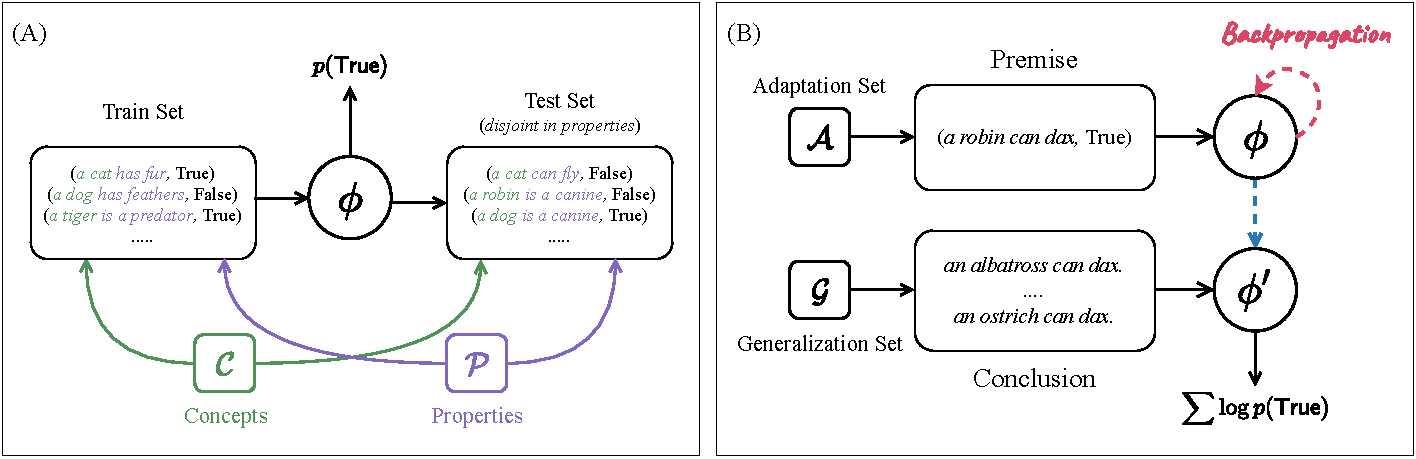
\includegraphics[width=0.8\textwidth]{inductionframeworkcogsci.pdf}
    \caption{\textbf{(A)} Property Judgment Stage describing the training of the property judgment model $\phi$ to make judgments of truth on sentences expressing concept-property assertions. Sentences created using the concept ($\concepts$) and property ($\properties$) data collected by \citet{devereux2014centre}; \textbf{(B)} Depiction of the Induction Stage, in this case, for testing the generalization from robin to all birds. Here, $\adaptation = \{\textsc{robin}\}$, $\generalization = \{\textsc{albatross}, ..., \textsc{ostrich}\}$, and the novel property being generalized is ``\textit{can dax}.''}
    \label{fig:framework}
\end{figure*}
\subsection{Stage 2: Induction as Domain Adaptation}
% We operationalize induction as 
In this stage, we use the fine-tuned model from the previous stage to perform property induction, which we operationalize as the adaptation of the model to new property knowledge via backpropagation \citep{rumelhart1986learning}.
The motivation to use backpropagation to perform property induction is simple -- it allows the integration of new information in the model by directly interacting and updating its representations which seemingly encode knowledge that is used to inform how the model generalizes. 
This integration is numerical and therefore measurable by using metrics such as loss or accuracy, which allows us to shed light on how well the model integrates certain kinds of knowledge.
A similar operationalization of induction was used by the pioneering work of \citet{rogers2004semantic}, who reported inductive inferences made by their PDP model of semantic cognition by updating its weights to reflect novel information which was provided after several steps of training on general conceptual knowledge derived from a toy-dataset of concepts and properties.
Similarly, \citet{van2018neural} adapt language models on novel syntactic structures to shed light on their syntactic adaptation capacities.

An instance of property induction involves: (1) a set of premise concepts (which we denote as the adaptation set $\adaptation \subset \concepts$); (2) a set of conclusion concepts (denoted as the generalization set $\generalization \subset \concepts$); and (3) a novel property being generalized from the premise to the conclusion.
% The content of these artifacts depends on the specific inductive phenomena being simulated.
We construct sentences that associate the novel property to the concepts in $\adaptation$ and $\generalization$, yielding the premise and conclusion stimuli, respectively (see Figure 1B)
To perform a round of property-induction, we first adapt the model $\phi$ to the premise sentences by using standard backpropagation, yielding an updated state of the model $\phi^{\prime}$, that correctly attributes the concepts in $\adaptation$ with the novel property.
We then freeze the parameters of $\phi^{\prime}$ and query it with the conclusion sentences to get the model's (log) probability of generalizing (or ``projecting'') the novel property to the concepts in $\generalization$.
An example of this stage is shown in \Cref{fig:framework}B.
% To formalize this notion, we denote the source concepts by $S$
% While every induction experiment is idiosyncratic to the phenomena of interest, we will use \cref{arg:example} as the running example.
% \km{backpropagation as mechanism to integrate new knowledge into the representations of model obtained in the previous stage.}
% \subsection{Using the Framework}
% To measure the strength of projecting the novel property to a given set of generalization concepts, we use log-probabilities from the updated model $\phi^{\prime}$
% An instance of property induction can involve the testing of generalization to one or more concepts.
We denote the model's log-probability on the generalization set as the ``generalization score'' ($\mathbb{G}$) -- the strength of projecting the novel property to a set of one or more concepts in the generalization set:
% We compute the argument strength for instances with single concept in the generalization set as:
% \begin{align*}
%     AS = \log p_{\phi^{\prime}}(\textit{``c}\textit{ has property X''} = \true)
% \end{align*}
% For cases when the generalization set consists of multiple concepts (e.g., superordinate categories such as \textsc{bird}),
% It is computed as the average log-probability of generalizing the novel property to all concepts in the generalization set:
\begin{align}
    \mathbb{G} = \frac{1}{n}\sum_{\textit{c}_i \in \mathcal{G}} \log p_{\phi^{\prime}}(\textit{``c}_i\textit{ has property X''} = \true)\label{eq:genscore}
\end{align}

We now use components of this framework in two experiments -- one for each stage in the framework.

\section{Property Judgment Experiment}
This experiment focuses on the first stage of the proposed induction framework. Here, we fine-tune pre-trained LMs to judge the truth of sentences that link concepts to properties. 
Since our setup keeps the training and the evaluation data perfectly disjoint in terms of properties (as we will show), a model will \textit{have} to constrain its parameters to rely on property knowledge in order to succeed -- we therefore test the extent to which this indeed is the case. 
\paragraph{Property Knowledge Data}
To construct sentences that express property knowledge, we rely on a property-norm dataset collected by the Cambridge Centre for Speech, Language, and the Brain \citep[CSLB;][]{devereux2014centre}.
The CSLB dataset was collected by asking 123     human participants to elicit properties for a finite set of 638 concepts, and has been used in several
% a number of 
studies focused on investigating conceptual knowledge in word representations learned by computational models of text \citep[e.g., ][]{lucy-gauthier-2017-distributional, da-kasai-2019-cracking, bhatia2020transformer}.
Property-norm datasets consists of data about what properties are possessed by a given concept and therefore lack negative concept-property associations. 
As a result, the aforementioned works randomly sample concepts for which a particular property was not elicited and take them as negative instances, which can then be used in a standard machine-learning setting to evaluate a given representation-learning model.

% \ake{The description of all of this data cleaning maybe belongs in its own section, if it's not a part of this experiment per se?} 
Upon careful inspection of the CSLB dataset, we found that the above practice may unintentionally introduce incorrect data, and affect the conclusions of previous works.
Datasets such as CSLB are collected through human elicitation of properties for a given concept, so it is possible that there are cases when a property was not elicited for some concepts -- we suspect this may happen when some participants chose not to elicit properties that were obvious to the presented concept (e.g., \textit{breathing} in case of living organisms), while other participants did, resulting in an imbalance that was left unaccounted.
We found that this was indeed the case -- e.g., the property \textit{has a mouth} was only elicited for 6 animal concepts (out of 152), and so all other animals in the dataset would have been added to the negative search space during sampling, thereby propagating incorrect and incomplete data. This indicates a potential pitfall of directly using property-norm datasets to investigate semantic representations, suggesting that prior evaluations and analyses \citep{lucy-gauthier-2017-distributional, da-kasai-2019-cracking, bhatia2020transformer} may have falsely rewarded or penalized models in some cases.
To mitigate this issue, we first selected the categories \citep[hand-annotated by][e.g., \textsc{bird, vehicle, tree}, etc.]{devereux2014centre} that had at least 9 concepts in the dataset and were not labelled as ``miscellaneous,'' resulting in 24 different categories with a total of 538 unique noun concepts, and 4{,}970 unique properties.
Next, we manually removed concepts and properties that contained proper-nouns (e.g., \textsc{rolls-royce}, \textit{is in Harry Potter}), stereotypical or subjective data (e.g., \textit{is meant for girls}, \textit{is ugly}), and explicit mentions of similarity or relatedness (e.g., \textit{is similar to horse}). We further normalized properties that were paraphrases of each other (e.g., \textit{is used to flavor, does flavor} $\rightarrow$ \textit{is used to flavor}). This resulted in 530 concepts and  3{,}873 properties.
Again through manual annotation, we identified a total of 234 properties that were incompletely annotated (i.e., those that were possessed by certain concepts but were not elicited during data collection, e.g., \textit{can grow} missing for all invertebrates) and extended their coverage. 
While this may seem like a small number (6\% of the valid properties), it greatly increases the total number of concept-property pairs (from 13{,}355 pairs to 22{,}046, an increase of 65\%), since many of the incompletely labelled properties were applicable across several categories.
-- e.g., \textit{has a mouth, can grow,} etc.

% Using the 530 concepts ($\concepts$) and 3{,}873 properties ($\properties$), we generate 
Instead of randomly sampling negative concepts for each of our 3{,}873 properties ($\properties$), we sample concepts are that are similar to those that possess a particular property -- e.g., for the concept \textsc{zebra}, we want to use \textsc{horse} as a negative sample over something random such as \textsc{table}.
By doing so, we make the property judgment tasks increasingly difficult, increasing the chances that the models that we obtain after this stage are indeed focusing on conceptual knowledge to make property judgments instead of relying on simpler superficial cues such as lexical co-occurrence \citep{mccoy-etal-2019-right}.  
To this end, we first create a taxonomy of our 530 concepts ($\concepts$) by identifying their WordNet \citep{miller1995wordnet} senses.
Then, for each property---associated with $k$ different concepts that possess it---we perform a weighted sampling from the set of leftover concepts (with size $530 - k$), where each leftover concept is assigned a weight proportional to its \textit{Wu-Palmer similarity} \citep[a commonly used taxonomic similarity computed over the subset of wordnet taxonomy;][]{wu-palmer-1994-verb} with every concept that possesses the property. 
This results in a set of negative concept-property pairs that is equal in size to our positive set.
We then follow the method outlined by \citet{bhatia2020transformer} to convert our concept-property pairs into 22{,}046 true and 22{,}046 false property knowledge sentences.
% \footnote{this involves minimal modification since most of our properties are already represented as well-formed verb-phrases.}
Finally, we split our 44{,}092 sentence-label pairs into training, validation, and testing sets (80/10/10 split), such that the testing and validation sets are only composed of properties that have never been encountered during training, and are also disjoint from each other. 
We do this to avoid data-leaks, and ensure that we evaluate models on their capacity to learn property judgment as opposed to memorization of the task.
We make our entire filtering pipeline and negative sample generation algorithm available in our code (url hidden).

\paragraph{LMs used}
While our framework can be applied to any neural language model, we specifically present results from fine-tuning three selected pre-trained LM families, based on the precedence of using them in standard sentence classification tasks \citep{wang2018glue}: BERT \citep{devlin-etal-2019-bert}, RoBERTa \citep{liu2019roberta}, and ALBERT \citep{lan2019albert}. 
% The models were selected on the basis of their \km{(preferred)} use in standard sentence classification tasks in the NLP community \citep{wang2018glue}. 
All three models use the transformer architecture \citep{vaswani2017attention}, and are trained to perform masked language modeling -- the task of predicting words in context in a cloze-task setup, where they have access to words to the left and right of the masked word. 
We report results using the largest models in each of the three families---BERT-large, RoBERTa-large, and ALBERT-xxl---since they had the best performance in our preliminary experiments.
% \paragraph{Fine-tuning}
We fine-tune each of the three models on the property knowledge data by minimizing their binary cross-entropy loss on the training set using the Adam optimizer \citep{kingma2014adam}.
We tuned the hyper-parameters (such as learning rate) on the basis of the validation set, and finally evaluated the three adapted models on the test set using the F1 score.
% Let $\mathcal{C}_{\properties_i}^{\prime}$ be the set of concepts that do not possess a particular property $\properties_i$
% Then, for each property, we first split $\concepts$
% \begin{align}
%     \frac{(n+1)\times \texttt{depth}(\texttt{lcs}(p_1, \dots, p_n, r_i))}{\texttt{depth}(p_1) + \dots + \texttt{depth}(p_n) + \texttt{depth}(r_i)}
% \end{align}
% In order to get models that are more conducive to rely on conceptual knowledge to make property judgments instead of superficial cues \citep{mccoy-etal-2019-right}, we 

% \km{CSLB norms \citep{devereux2014centre} consisting of n concepts and m properties. How this dataset has traditionally been used in probing experiments -- for each category, all members that do not have an associated production frequency are set to False. Upon careful inspection, we find that this practice can introduce unintended problems -- ``absence of evidence vs. evidence of absence''}

% \km{Train test split creation: negative instances created by sampling similar concepts that do not possess the properties, using a taxonomic similarity metric (details in supplementary material)}

\paragraph{Results}
\Cref{tab:f1} shows the performance of the three models from our property judgment experiments. 
% \km{generally high scores, suggesting that to an extent the model learn to rely on concept knowledge through this true-false setup.}
We find that all three models show approximately similar validation (between 0.79 - 0.82) and test performance ($\approx$ 0.79 throughout), suggesting strong capacities of all three models in assessing the application of properties to concepts. Notably, the ALBERT-xxl model shows the same performance as BERT-large and RoBERTa-large despite having $\approx$130M fewer parameters, highlighting its efficient use of parameters.

\begin{table}[t!]
\vspace{-1em}
\def\arraystretch{1.15}
\centering
\caption{Performance (F1 scores) of the three adapted models on Validation and Test sets, each of which is disjoint in terms of properties from the Training set. Chance F1 = 0.50}
\label{tab:f1}
\vspace{0.5em}
\begin{tabular}{|l|c|c|c|}
\hline
\textbf{Model} & \textbf{Params} & \textbf{Val. F1} & \textbf{Test F1} \\ \hline
ALBERT-xxl     & 212M            & 0.81             & 0.79    \\
BERT-large     & 340M            & 0.79             & 0.79    \\
RoBERTa-large  & 345M            & 0.82    & 0.79    \\ \hline
\end{tabular}
\end{table}

\section{Investigating Taxonomic Generalizations in LMs using Property Induction}
% Using the three property-judgment models from the previous experiment, we now demonstrate how our induction framework can be used to answer questions related to the models' inductive behavior, and by extension the kinds of knowledge they may be putting to use in making generalizations beyond available data.
% As a case-study, we will focus on inductive generalizations made on the basis of taxonomic relations between concepts and ask whether the models use knowledge of category-membership to make project newly provided properties.
The taxonomic relation between concepts has an important role in studies of human inductive reasoning.
Early evidence from \citet{gelman1986categories} indicated a strong preference of children and adults in making generalizations about new and unfamiliar properties consistent with the structure of biological taxonomies and category-membership.
\begin{figure*}[h]
    \centering
    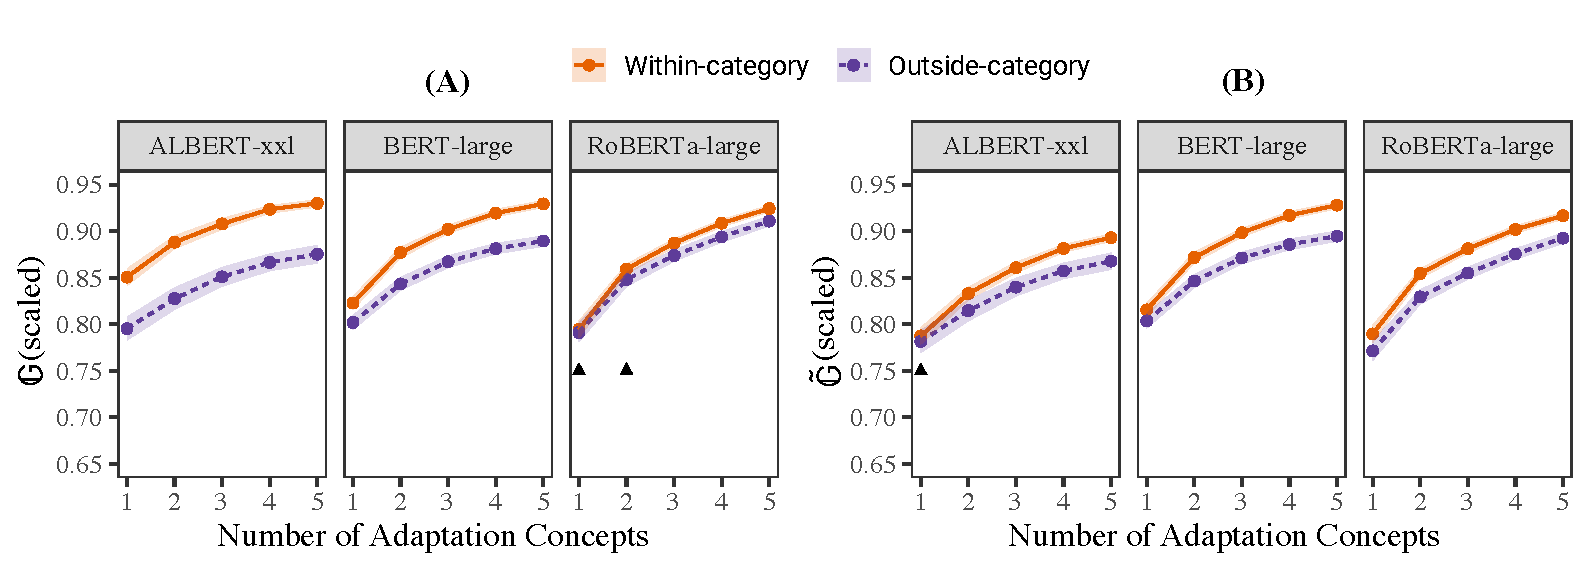
\includegraphics[width=0.9\textwidth]{withwithoutoverlaps.pdf}
    \caption{\textbf{(A):} Results from Taxonomic Generalization experiment showing generalization scores ($\mathbb{G}$) between ``Within-category'' and ``Outside-category'' generalization sets across various number of adaptation concepts. \textbf{(B):} Same depiction as \textbf{(A)} but with the the effect of property-overlaps between adaptation and generalization concepts removed. Cases where the difference between $\mathbb{G}$-scores of within versus outside category sets are not significant under $\alpha = .05$ are marked with a `$\blacktriangle$'}
    \label{fig:taxonomicresults}
\end{figure*}
% \citet{gelman1986categories} were one of the first ones to observe the role of taxonomic relations emerge in patterns of induction in children and adults. 
% In their experiments, \citeauthor{gelman1986categories} first displayed a picture of a flamingo to their subjects and informed them that it had a ``right aortic arch,'' then displayed a picture of a bat and told them that it had a ``left aortic arch.'' 
% When later shown a picture of a blackbird (that visually resembled the bat more than it did the flamingo), the subjects attributed it ``a right aortic arch'', indicating a preference for biological taxonomies in their inductive judgments.
Building on this, \citet{osherson1990category} documented 13 separate taxonomic phenomena that influenced inductions made by humans.
Inspired by these pioneering works, we demonstrate how our property induction framework can be used to test whether a similar taxonomic bias is acquired by the models (obtained from the previous experiment). 
For instance, if a model is provided with a new property---e.g., \textit{can fep}---that is associated with the concept \textsc{cat}, to what extent does it prefer generalizing or projecting it to all mammals?
% Furthermore, the notion of \textit{premise monotonicity} \citep{osherson1990category} suggests that the inductive strength of ``\textit{all mammals can fep}'' should increase with an increase in the number of premise concepts (i.e., the generalization score for \{\textsc{cat}, \textsc{cow}\} to mammals should be greater than that from \textsc{cat} to mammals). 
We shed light on whether the representations of the three property judgment models support generalizations that are made on the basis of category-membership using an experiment where models are provided with new properties about existing concepts, and are then subjected to analyses which test the extent to which they project the new property to concepts that lie within---as opposed to outside--- the same category as the input.


\paragraph{Data} We restrict our analysis to the animal-kingdom subset of the concepts in our modified property-norm data, corresponding to a total of 152 concepts.
We first select the top six categories within this subset -- \textsc{mammal} (52), \textsc{bird} (36), \textsc{insect} (18), \textsc{fish} (14), \textsc{mollusk} (8), and \textsc{reptile} (7).
Each instance in this experiment starts with a focus category (of size $m$) from which we sample $n$ concepts to create the adaptation set, and use the remaining $m-n$ to create the ``Within-category'' generalization set.
Similarly, we create the ``Outside-category'' generalization set by sampling the top $m-n$ animal concepts that are outside the focus category, on the basis of their average cosine similarity with the concepts in the adaptation set (calculated using the representations from the embedding layer of the given model). We use this weighted sampling technique in-lieu of simple random sampling to test differences between within and outside category generalization at their intuitive limits -- 
% it is reasonable to assume that representational similarity may play a role in the model's generalizations, so 
having our outside-category set be similar to the adaptation set as opposed to being randomly sampled allows us to be more confident in our conclusions.
We repeat this sampling process 10 times, for $n = 1, \dots, 5$ adaptation concepts, and 8 novel properties -- verb-phrases created using nonce words (\textit{can dax, can fep, has blickets, has feps, is a tove, is a wug, is mimsy, is vorpal}). In total, we have 2{,}400 samples per model.
%$6 \times 10 \times 5 \times 8 = 2400$
\paragraph{Method}
In each trial, we pass the adaptation set to the models and let them minimize their loss---using the same optimizer state as the one obtained at the end of the property judgment task---until they reach perfect accuracy. Then for each model, we compute $\mathbb{G}$ for both our generalization sets as shown in \cref{eq:genscore}. 
\Cref{fig:taxonomicresults}A shows the average $\mathbb{G}$ (over all properties, re-scaled to lie between 0 and 1) across the number of adaptation concepts.

\paragraph{Results and Analysis}
It is expected that models with a preference towards category-membership will have greater average $\mathbb{G}$ values for the ``Within-category'' set than for the ``Outside-category'' set.
From \Cref{fig:taxonomicresults}A, we observe ALBERT-xxl and BERT-large to consistently 
show this pattern (differences between ``Within-category'' and ``Outside-category'' were significant at $p<.001$ using a t-test). This preference is substantially lower for RoBERTa-large (with non-significant differences between generalization to within versus outside category for $n=1,2$), highlighting its near-indifference to taxonomic vs. representational similarity in extending new property knowledge to concepts outside the adaptation set.
Furthermore, we observe that the average generalization score in both categories increases with an increase in the number of adaptation concepts. While this is also robustly observed in humans (characterized as the \textit{premise monotonicity effect} by \citeauthor{osherson1990category}), it is expected that data-driven models are likely to be more confident in their outputs as the number of samples provided to them increases.

Although the properties provided to the model are ones they have never seen during training (i.e., in the property-judgment stage), to what extent can the models' inductive behavior be explained by the overlap in properties between the concepts of the adaptation set and each of the generalization sets? Under the connectionist perspective of property induction \citep{sloman1993feature, rogers2004semantic}, the strength of generalization (of a novel property) to a concept is proportional to the overlap in properties between the premise (adaptation set) and the conclusion (generalization set).
We can reasonably expect this to translate to the models that we use here,
% ---they essentially are sophisticated successors of connectionist models---
especially since they are trained to predict the presence and absence of properties.
It is therefore revealing to understand the extent to which the models' preference towards category-membership persists when the component of their generalizations that is attributable to the property overlaps in the training set is no longer present.
To this end, we  predict each model's generalization scores ($\mathbb{G}$) using the overlap of properties ($o$, computed as proportion of common properties) between the concepts of the adaptation set and that of the generalization set. We then regress out the relationship between $\mathbb{G}$ and $o$ to obtain the adjusted generalization scores ($\Tilde{\mathbb{G}}$):
\begin{align*}
    \mathbb{G}_i &= \beta_0 + \beta_1 o_i + \epsilon_i\\
    \Tilde{\mathbb{G}}_i &= \mathbb{G}_i - \beta_1 o_i = \beta_0 + \epsilon_i \tag{adjusted $\mathbb{G}$}
\end{align*}
\Cref{fig:taxonomicresults}B shows the $\Tilde{\mathbb{G}}$ scores (re-scaled to be between 0 and 1) for each model and across different number of adaptation concepts.
% while the relative difference in patterns of generalization for BERT-large roughly remained the same,
We observe that there were notable changes in patterns of generalization for ALBERT-xxl (decrease in difference) and RoBERTa-large (decrease in difference). 
This suggests that property-overlaps had a positive-effect on the generalizations made by ALBERT-xxl ($R^2=0.055, \beta_1 = 0.86, p < .001$) and a negative-effect on those by RoBERTa-large ($R^2=0.007, \beta_1 = -0.17, p < .001$). Although the effect of property-overlaps was positive for BERT ($R^2=0.004, \beta_1 = 0.13, p < .001$), the differences before and after the adjustment were too small to notice. 
Notably, in all models, property-overlaps were only able to account for a small percent of variance ($0.4\%$ to $5.5\%)$, suggesting that the models were likely using information that is different from simple training-set overlaps to perform property induction.
Overall, the general trend in models' preference to generalize to ``Within-category'' over the ``Outside-category'' persisted in almost all cases (except for ALBERT-xxl, $n=1$), suggesting the presence of a \textit{taxonomic bias} in these models, even when the effect of property-overlaps was removed.


\section{General Discussion and Conclusion}
% \km{Investigations focused on }
% Studies of human property induction \citep{gelman1986categories, carey1985conceptual, osherson1990category} shed light on how humans use their intuitive understanding of the world to deploy novel information about concepts and properties.
The empirical success of neural network-powered language models (LMs)---especially on high-level semantic tasks---has lent further support to the study of language as a source of semantic knowledge \citep{elman1990finding, lupyan2019words}.
A number of works have since sought to understand the ability of LMs to recall conceptual knowledge in a word-prediction setup \citep{petroni2019language, weir2020probing, misra2021typicality}, or by analysing whether individual property information can be decoded from the models' representations \citep{lucy-gauthier-2017-distributional, forbes2019neural, bhatia2020transformer}.
The goal of this paper was to extend this line of inquiry by understanding the ways in which LMs generalize novel property information (\textit{a lion can fep}) beyond their training experience.
To this end, we developed a framework that used LMs to perform \textit{property induction} -- a paradigm through which cognitive scientists have studied how humans use their conceptual repertoire to project novel information about concepts and properties in systematic ways.
By simulating a similar process in LMs, our framework can yield insights about the inductive preferences that are reflected in the LMs representations as well as shed light on the nature of the models' knowledge of concepts and their properties.

As a motivating case-study, we used our property induction framework to study the extent to which LM representations showed a preference to project novel properties on the basis of category-membership. 
% That is, we tasked models to project a novel property that was associated with one or more concepts (up to five) and compared their projection of the property between a set of concepts that lied in the same category as the input, and an independent set of concepts with high representational similarity as the input.
To this end, we adapted the LM representations---fine-tuned to explicitly predict the truth of sentences expressing property knowledge---to inputs where a novel property was associated with one or more concepts. We then compared their projection of the novel property between (1) a set of concepts that were in the same category as the input, and (2) an independent control-set of concepts that had high-representational similarity as the input.
In majority of cases, models consistently preferred to project the new property to former, suggesting the likely presence of a taxonomic bias in them.
% Recall that the models that we used in these experiments were trained to predict the truth of sentences that linked concepts to properties. 
We hypothesized that one reason why models may have preferred to generalize within the input's taxonomic category could be due to high overlap of properties between the input concepts and those that lied in the same category. 
While property-overlaps were statistically predictive of how models projected novel properties, the preference to generalize them  to concepts within---as opposed to outside---the category persisted even when this predictive effect was removed.

% Our taxonomic generalization results suggest that models may have learned to use category-membership knowledge in projecting new information, they also lead to a number of outstanding hypotheses that can be tested using our framework.
% One hypothesis comes from the observation that models displayed a taxonomic bias even when the predictive component of training-set property overlaps was removed. 
Our results indicate that the models are likely going beyond simple training-set overlaps to project novel property knowledge.
This leads to two broad hypotheses that can further explain this behavior at a deeper level.
One hypothesis could be that the models are using only a subset of overlapping properties that are dynamically activated based on the interaction of the type of property and the input and generalization concepts -- for instance, models may use a different subset of properties to generalize \textit{can} versus \textit{has} properties \citep{rogers2004semantic}.
Another hypothesis is that these models could also be using knowledge that is outside the training set but is implicitly activated as a result of fine-tuning. 
This hypothesis is supported by the models' decent performance on the disjoint test and validation sets in our property judgment experiment -- where the models' ability to judge the truth of sentences expressing property knowledge that they had never encountered was substantially above chance.
The test of whether or not models are sensitive to a property present outside their training experience can readily be conducted using our framework.
% This hypothesis can readily tested using our framework readily allows the testing of whether models are sensitive to implicit properties not present in their property judgment training. 
In this case, we can design adaptation sets that implicitly encode a given property that is not present in the training set -- e.g., the property of \textit{flight} is implicitly available as \textit{has X} in the set \{(\textit{robin has X}, True), (\textit{emu has X}, False), (\textit{butterfly has X}, True)\}. We can then test the extent to which the model makes generalizations consistent with the implicit property by comparing its output on \textit{bee has X} versus \textit{penguin has X}. A model that has successfully recognized the presence of the implicit property will assign higher generalization score to the former.
% -- i.e., a model that has successfully recognized the presence of \textit{can fly} in this example should assign greater probability to \textit{bee has X} as compared to \textit{penguin has X}.
We hope to test these hypotheses and the models' capacity to implicitly use salient properties in future work.

% Our results can potentially inform a number of future experiments. For instance, our results before and after removing the effect of property overlap
% to test whether they acquired a preference to generalize new information on the basis of category-membership. Our results in the induction task indicated that model likely possessed a taxonomic bias in }


\bibliographystyle{apacite}

\setlength{\bibleftmargin}{.125in}
\setlength{\bibindent}{-\bibleftmargin}

\bibliography{CogSci_Template}

% \clearpage

% \appendix

% \section{Algorithm for Constructing Negative Instances}


\end{document}
